\documentclass{beamer}
\usepackage{ctex, hyperref}
\usepackage[T1]{fontenc}

% other packages
\usepackage{latexsym,amsmath,xcolor,multicol,booktabs,calligra}
\usepackage{graphicx,pstricks,listings,stackengine}

\author{Lucas Astor, Micalea Olivera, Valentina Ribas, Diego Bergara}
\title{Defensa segundo trabajo practico}
\subtitle{Probabilidad y Estadistica}
\institute{UNIVERSIDAD CATOLICA DEL URUGUAY}
\date{2021 11 23}
\usepackage{SDU}

% defs
\def\cmd#1{\texttt{\color{blue}\footnotesize $\backslash$#1}}
\def\env#1{\texttt{\color{blue}\footnotesize #1}}
\definecolor{deepblue}{rgb}{0,0,0.5}
\definecolor{deepgreen}{rgb}{0,0.5,0}
\definecolor{halfgray}{gray}{0.55}

\lstset{
    basicstyle=\ttfamily\small,
    keywordstyle=\bfseries\color{deepblue},
    emphstyle=\ttfamily\color{deepblue},    % Custom highlighting style
    stringstyle=\color{deepgreen},
    numbers=left,
    numberstyle=\small\color{halfgray},
    rulesepcolor=\color{blue!20!green!20!blue!20},
    frame=shadowbox,
}


\begin{document}

\kaishu

\begin{frame}
    \titlepage
    \begin{figure}[htpb]
        \begin{center}
            
\includegraphics[width=0.2\linewidth]{pic/logo.png}
        \end{center}
    \end{figure}
\end{frame}

\begin{frame}
    \tableofcontents[sectionstyle=show,subsectionstyle=show/shaded/hide,subsubsectionstyle=show/shaded/hide]
\end{frame}


\section{Ejercicio 1}


\begin{frame}{Esperanza y Varianza}
    \begin{exampleblock}{Ecuaciones}
        % Taken from Mathmode.tex
        \begin{multline}
            Esperanza = E\left(\overline X_{n})=\right.E\left(X_{1})\right., Varianza = V\left(\overline X_{n})=\right.\frac{V\left(X_{n})\right.}{n}\label{eq:reset}\\
            E\left(\overline X_{50})=\right. E\left(X_{1}) \right. siendo \left(X_{1})\sim \right. N\left(-4, 16)=\right. -4\\
            V\left(\overline X_{50})=\right.\frac{V\left(X_{1})\right.}{50} siendo \left(X_{1})\sim \right. N\left(-4, 16)=\right. \frac{16}{50} = 0,32 \label{eq:reset}\\
        \end{multline}
    \end{exampleblock}
\end{frame}


\begin{frame}{Histograma}
    \begin{itemize}[<+-| alert@+>] % 当然,除了alert,手动在里面插 \pause 也行
        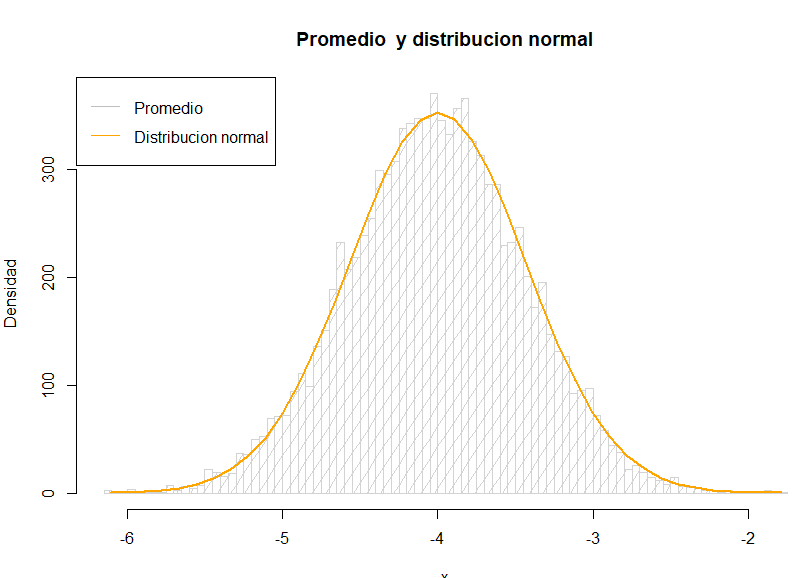
\includegraphics[width=0.99\linewidth]{pic/histograma.png}
    \end{itemize}
\end{frame}

\begin{frame}[fragile]{\R{} Codigo utilizado para HISTOGRAMA}

\begin{lstlisting}[language=R]
 hist(vPromedios, breaks = 100, density = 10) 
 seq(min(vPromedios), max(vPromedios), length=40)
 dnorm(xfit, mean = -4, sd =sqrt(0.32))

\end{lstlisting}
    \medskip
    \pause
\end{frame}


\end{document}
